%!TEX root = notas_de_clase.tex


\section{Support Vector Machines}

\subsection{Introducción}
\label{sub:svm_intro}

En este capítulo del apunte, discutiremos las llamadas \textbf{máquinas de soporte vectorial} (SVM) que constituyen un set de herramientas para resolver el problema de clasificación de datos. Fue desarrollada en los 90 dentro de la comunidad de computer science y ha crecido enormemente desde entonces. Esta técnica ha demostrado ser útil en diversos escenarios, y es considerado uno de los mejores clasificadores para ``llegar y usar''. 

\subsection{Idea general}


Los SVM son una generalización de un clasificador más simple e intuitivo llamado el clasificador de márgen máximo (\textit{maximum margin classifier})

Para estudiar dicho clasficador, comenzaremos estudiando el caso en que tenemos que clasificar los datos en dos grupos, y además supondremos que los datos son linealmente separables (es decir, existe un hiperplano que los separa, ver fig.~\ref{fig:maxim_marg}). Esto último es claramente un supuesto muy fuerte, pero lo generalizaremos mas adelante. 


\begin{figure}[ht]
    \centering
    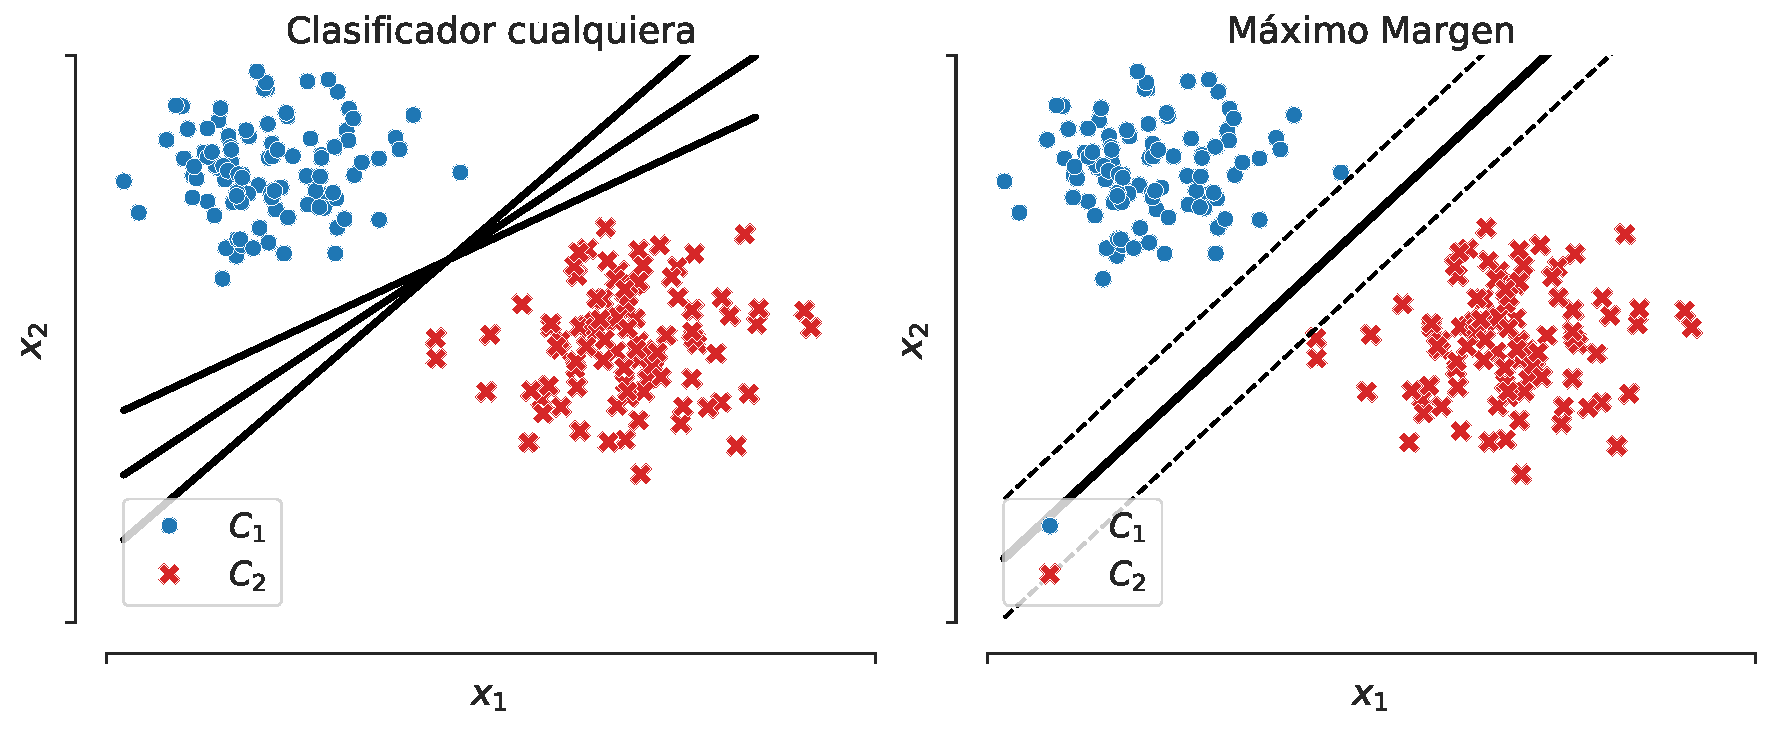
\includegraphics[width=0.9\textwidth]{img/cap5_max_margen.pdf}
    \caption{Modelo de máximo margen entre los datos}
    \label{fig:maxim_marg} 
\end{figure}


Como se puede apreciar en la fig.~\ref{fig:maxim_marg} (centro), dados puntos linealmente separables, existen diferentes hiperplanos que separan los datos. Cada una de estas líneas define un modelo, ya que dado un nuevo dato $x^*$, si este está por encima de la línea, entonces es un dato verde, en cambio si esta por debajo, entonces es un dato rojo. 
\\

¿Cuál elegir?
\\

Estudiaremos una respuesta natural al problema: ¿cómo elegir el hiperplano que nos entregue el \textbf{mayor margen} posible entre ambos grupos? Esto se traduce en reemplazar el problema de separar mediante una línea, en separar mediante una \emph{cinta} de ancho máximo. A este modelo se le llama el separador de máximo margen que mencionamos antes. 
\\

El argumento de ocupar dicho modelo es que uno esperaría que si un modelo tiene un buen margen en los datos de entrenamiento, entonces el \textbf{error de generalización} (Cuanto se equivoca el modelo con datos nuevos) debiese ser bajo. Existe un argumento matemático, y a grandes rasgos es que a mayor margen y a medida aumentan los datos,  podemos acotar la probabilidad de error (Al estilo desigualdad de Markov) sin embargo los detalles se escapan de los contenidos del curso.  
\\

Continuando, en la fig.~\ref{fig:maxim_marg} (derecha) podemos visualizar el modelo. Notar que el  margen esta definido solamente por algunos puntos. En la figura son dos, podrían ser más, pero nunca menos por la naturaleza `` simétrica '' del modelo.
\\

Dichos puntos que definen el márgen son llamados los vectores de soporte (support vectors) que le entregan el nombre al método. 
\\

Un ejemplo sencillo para recordar que es lo que hace SVM es imaginar que el ejemplo de los gráficos trata sobre clasificar manzanas y naranjas: 


A diferencia de otros métodos que aprenden analizando todos los datos y llegando a una respuesta (Cómo Naive Bayes, Regresión Lineal, etc...) de lo que en promedio podría ser una manzana, SVM mira la manzana mas naranjezca y la naranja mas manzanezca y con esos datos define un hiperplano separador. 



\begin{figure}[ht]
    \centering
    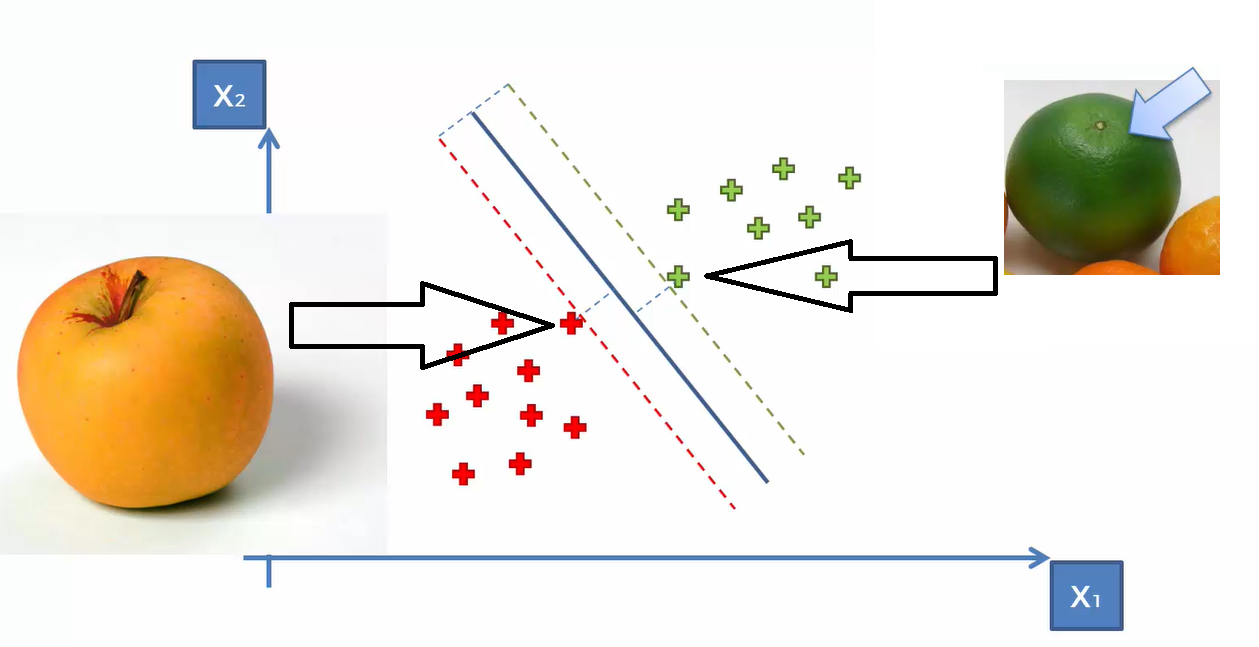
\includegraphics[scale=0.3]{img/img5.png}
    \caption{Los vectores de soporte son la manzana más naranjezca y la naranja más manzanezca}
    \label{fig:my_label1}
\end{figure}

\subsection{Problema}



Como ya mencionamos tenemos datos de entrenamiento $\{x_i\}_{1,...,N}$ que suponemos linealmente separables y deseamos encontrar un hiperplano de máximo margen que los separe. 

Un hiperplano en general son los $x\in \R^n$ que cumplan al ecuación

\begin{equation}
    w\cdot x + b = 0 
\end{equation}

Donde $w\in \R^n$ es el vector perpendicular al hiperplano y $b\in \R$ es un parámetro. La idea es encontrar $w$ y $b$ tales que entreguen el hiperplano separador de mayor margen. Este problema no tiene solución única (Pues si $w$ es solución entonces $\lambda w$ también). Para evitar ese problema, escalamos el plano de manera que los vectores de soporte ($x_{+}$ y $x_{-}$) sean tales que $w\cdot x_{+} + b = 1$ y $w\cdot x_{-} + b =  -1$ (Pueden haber mas vectores de soporte, pero para efectos del cálculo usaremos dos). Si bien aún no tenemos los vectores de soporte para hacer el escalamiento, este será parte de las restricciones del problema de optimización que resolveremos. 

El márgen del hiperplano es la mitad de la diferencia entre ambos vectores de soporte, proyectada en la dirección $\frac{w}{||w||}$ (Ver figura 5). 

\begin{figure}[ht]
    \centering
    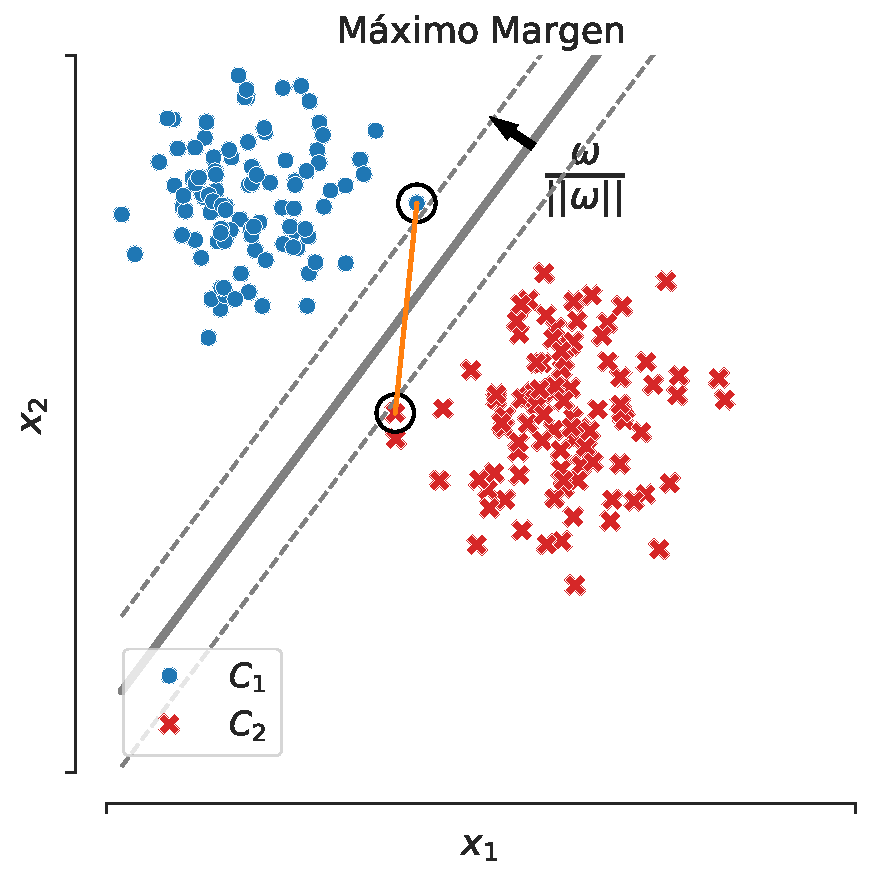
\includegraphics[width=0.4\textwidth]{img/cap5_max_margen2.pdf}
    \caption{En azul los vectores $x_+$ y $x_{-}$. En rojo el vector $(x_+ - x_{-})$. En naranjo la componente del vector rojo, proyectada en la dirección definda por $\frac{w}{||w||}$. Notar que corresponde justamente al doble del margen}
    \label{fig:my_label2}
\end{figure}

Calculamos:

\begin{align*}
    \frac{1}{2||w||}[ w \cdot (x_{+} - x_{-})] &= \frac{1}{2||w||} [ (w\cdot x_{+}) - (w\cdot x_{-})]\\
    &= \frac{1}{2||w||} [1 - (-1)]\\
    &= \frac{1}{||w||}
\end{align*}

Definiendo a $y_i$ como $1$ si $w\cdot x_i + b \geq1$ y $y_i =-1$ cuando  $w\cdot x_i + b \leq -1$, podemos formular el problema del hiperplano de margén máximo como

\begin{equation*}
\begin{aligned}
& \underset{w,b}{\text{max}}
& & \frac{1}{||w||}\\
& \text{s.a}
& & y_i (w\cdot x_i +b) \geq 1, \; i = 1, \ldots, N.
\end{aligned}
\end{equation*}

Para evitar problemas de diferenciablidad, en realidad se ocupa la siguiente formulazión equivalente

\begin{equation*}
\begin{aligned}
& \underset{w,b}{\text{min}}
& & \frac{1}{2}||w||^2\\
& \text{s.a}
& & y_i (w\cdot x_i +b) \geq 1, \; i = 1, \ldots, N.
\end{aligned}
\end{equation*}

Ahora estudiaremos el lagrangiano del problema (Y en consecuencia su dual). Este problema tiene una mejor estructura para optimizar, además que nos servirá para generalizar al caso no lineal. 

El lagrangiano es

\begin{equation*}
    L(w,b,\alpha) = \frac{1}{2}||w||^2 - \sum\limits_{i=1}^{N} \alpha_i (y_i (w\cdot x_i +b) -1)
\end{equation*}

Las condiciones de primer orden nos dicen que

\begin{equation}
    \dfrac{\partial L}{\partial w} = 0 \Rightarrow w = \sum\limits_{i=1}^{N} \alpha_i y_i x_i
\end{equation}

\begin{equation}
    \dfrac{\partial L}{\partial b} = 0 \Rightarrow \sum\limits_{i=1}^{N} \alpha_i y_i = 0 
\end{equation}


Reemplazando $(2)$ y $(3)$ en $L(w,b, \alpha)$, maximizando (por ser dual) e imponiendo holgura complementaria, el problema queda

\begin{equation*}
\begin{aligned}
& \underset{\alpha}{\text{max}}
& & \sum\limits_{i=1}^{N}\alpha_i - \frac{1}{2} \sum\limits_{i,j=1}^{N} \alpha_i \alpha_j y_i y_j \langle x_i, x_j\rangle\\
& \text{s.a}
& & \sum\limits_{i=1}^{N} \alpha_i y_i= 0 \\
& &  &\alpha_i \geq 0
\end{aligned}
\end{equation*}

Este problema es de la forma QP (Quadratic Programming) y existen diferentes métodos para resolverlo de manera óptima. 
Notar la participación del producto punto $\langle\cdot, \cdot\rangle$ en este problema, pues este será el punto de partida del SVM no lineal. 

Una vez resuelto el dual, la predicción de un nuevo punto $x^*$ es de la forma $$\hat{y}(x^*)= \text{sgn}\left(\left[\sum\limits_{i=1}^{N} \alpha_i y_i \langle x_i, x^*\rangle\right] - b\right)$$

Por holgura complementaria tenemos que si $x_i$ no está en el márgen, entonces $\alpha_i = 0$ de modo que $x_i$ no aporta en la predicción $\hat{y}$. Esta propiedad es la que mencionabamos al principio: La predicción solo depende de los vectores de soporte. 

Esta propiedad ayuda a resolver el problema de optimización de manera más rápida, ya que en realidad solo algunas variables duales $\alpha_i$ serán no nulas. Normalmente se ocupan heurísticas para encontrar rápidamente que vectores no son de soporte y así resolver un problema mas pequeño (Buscar, por ejemplo, el método de Sequential Minimal Optimization) 



\subsection{Soft Margin}


El planteamiento anterior tiene dos debilidades. Una, la más obvia, es que no siempre podemos tener datos separables y la segunda es que, incluso si los datos son linealmente separables, nuestro clasificador puede ser muy sensible a nuevos datos. Ver por ejemplo la Fig.\ref{fig:my_label3}.

\begin{figure}[ht]
    \centering
    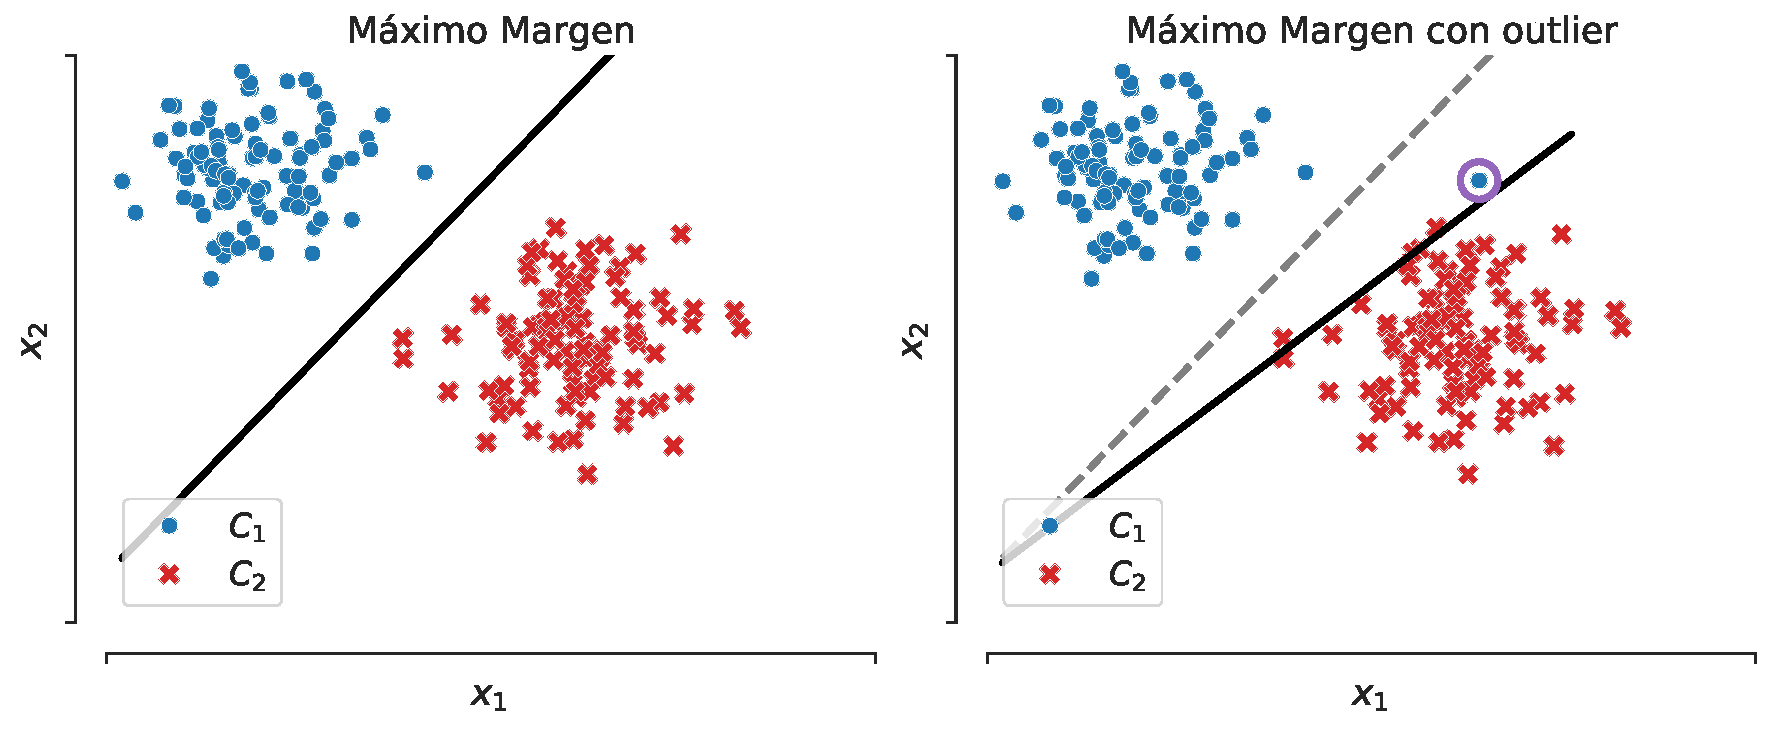
\includegraphics[width=0.9\textwidth]{img/cap5_margen_suave}
    \caption{Sensibilidad del máximo margen al agregar un nuevo dato.}
    \label{fig:my_label3}
\end{figure}


Como se ve en la imagen, la llegada del nuevo dato (encerrado en rojo) cambia drásticamente nuestro modelo. 

Para solucionar estos problemas (parcialmente) agregamos variables de holgura, que nos permitirán clasificar mal algunos datos. La idea es que, sacrificando algunos datos (muy probablemente outliers), podamos clasificar mejor la \textit{mayoría} de los datos (Clasificarlos todos era claramente muy ambicioso) y así tener un modelo mas robusto.  


Dicha formulazión del problema es la siguiente:

\begin{equation*}
\begin{aligned}
& \underset{w,b, \xi}{\text{min}}
& & \frac{1}{2}||w||^2 + c\sum\limits_{i=1}^{N} \xi_i \\
& \text{s.a}
& & y_i (w\cdot x_i +b) \geq 1 - \xi_i, \; i = 1, \ldots, N.
\end{aligned}
\end{equation*}

donde $c$ es un parámetro (Ya hablaremos de él).

Los $\xi$ indican que tan mal clasificado está un punto. Si $\xi_i = 0$, entonces el dato $x_i$ está al lado correcto del plano. Si $0<\xi_i <1$, entonces $x_i$ está al lado correcto del plano, pero viola la restricción del margen. Finalmente si $\xi_i>1$, entonces el punto esta al lado incorrecto del plano (Ver la siguiente figura)

\begin{figure}[ht]
    \centering
    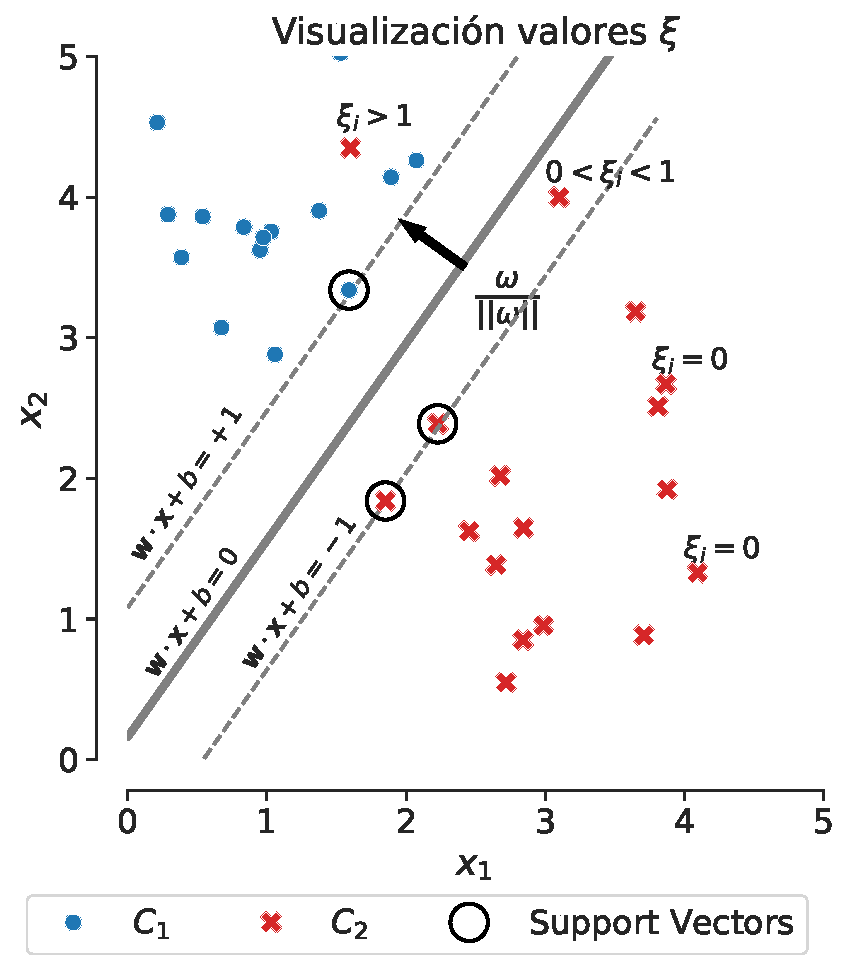
\includegraphics[width=0.45\textwidth]{img/cap5_max_margen3}
    \caption{Visualización de los valores de $\xi$}
    \label{fig:my_label4}
\end{figure}

El dual de este problema es (Usando Lagrangiano etc.)

\begin{equation*}
\begin{aligned}
& \underset{\alpha}{\text{max}}
& & \sum\limits_{i=1}^{N}\alpha_i - \frac{1}{2} \sum\limits_{i,j=1}^{N} \alpha_i \alpha_j y_i y_j \langle x_i, x_j\rangle\\
& \text{s.a}
& & \sum\limits_{i=1}^{N} \alpha_i y_i= 0 \\
& &  &0 \leq \alpha_i \leq c
\end{aligned}
\end{equation*}

Volveremos a este dual cuando veamos métodos no lineales. 
\\

Por último, ¿Qué hacer con el parámetro $c$? Guarda relación con el \textit{bias-variance tradeoff}. La variable $c$ es un parámetro de tolerancia. A mayor $c$, encontraremos un mayor márgen, lo que significa que nuestro modelo no estará sumamente ajustado a los datos (Lo que lo vuelve mas insesgado), pero probablemente se equivoque más (Tenga mayor varianza). Al revés, un $c$ muy pequeño nos llevará más cerca del caso inicial, donde nuestro margen será más pequeño, y por ende, raramente violado (Poca varianza), pero nuestro modelo podría quedar sobreajustado a nuestros datos, logrando un mayor sesgo.En la práctica se usa \textit{cross-validation} para encontrar un buen parámetro $c$.  


\subsection{Kernel Methods}

Los métodos anteriores se ven interesantes, pero podría desmotivar el hecho que sólo funciona para datos linealmente separables (Con un poco de holgura en el caso de soft margin). 

Un caso particular es el problema de clasificación XOR que se muestra en la siguiente figura

\begin{figure}[ht]
    \centering
    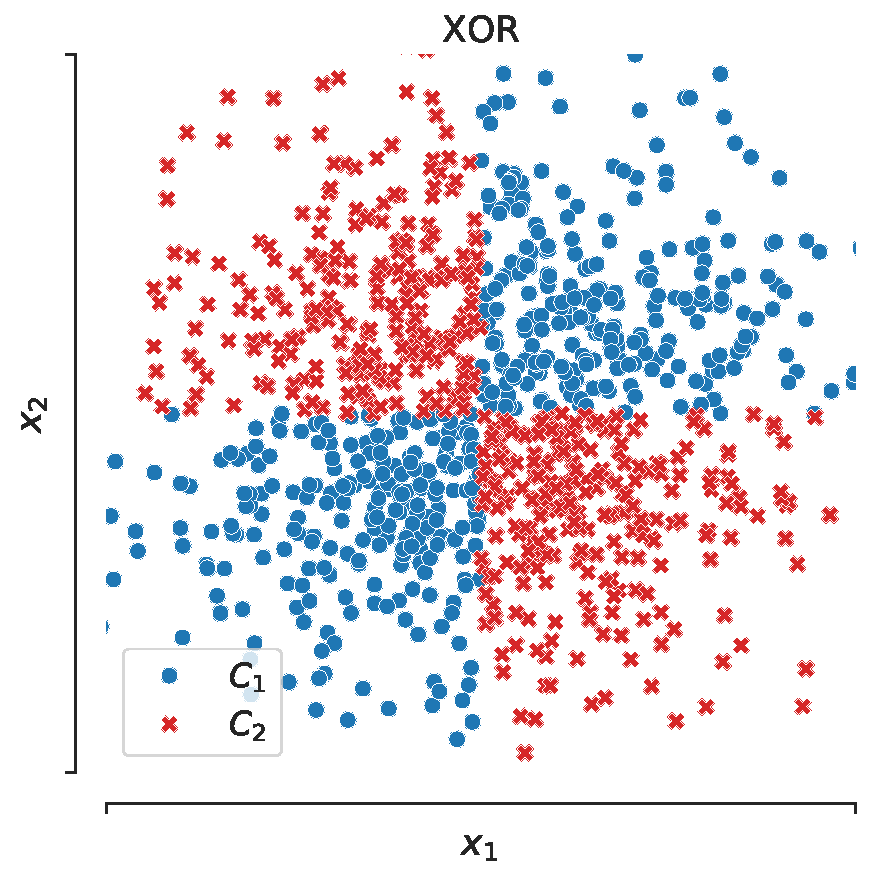
\includegraphics[width=0.45\textwidth]{img/cap5_xor}
    \caption{Datos XOR no son linealmente separables}
    \label{fig:my_label5}
\end{figure}

Dichos datos no son linealmente separables en $\R^2$, pero si consideramos el siguiente mapeo a $\R^3$

\begin{equation}
    \phi(x_1, x_2) = (x_1, x_2, x_1 x_2)
\end{equation}

Entonces es claro que el plano $z=0$ en $\R^3$ será capaz de separar dichos puntos (Pues si $x_1 x_2 > 0$ entonces dicho punto será rojo y estará por sobre el plano $z=0$, y análogamente sucede algo similar con los puntos azules). 

\begin{figure}[ht]
    \centering
    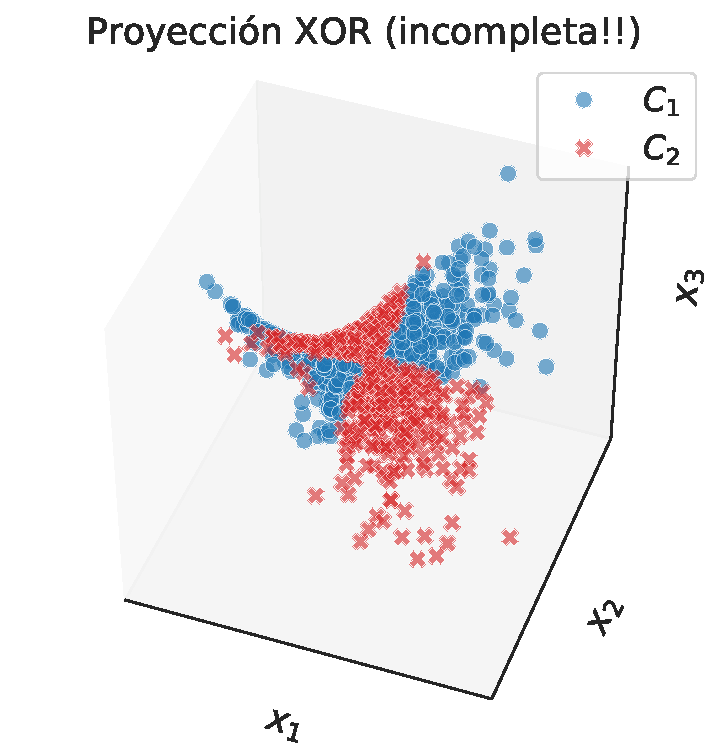
\includegraphics[width=0.45\textwidth]{img/cap5_xor_3d_proyeccion}
    \caption{Los puntos rojos y azules corresponden a los datos mapeados a través de $\phi$. El plano $z=0$ es claramente capaz de separar puntos rojos y puntos auzles en este nuevo espacio.}
    \label{fig:my_label6}
\end{figure}

%%VOLVER A PROYECTAR

La función $\phi$ se conoce normalmente como \textbf{feature map}. Es decir una función que entrega ciertos atributos de los datos (En este caso, por la forma del problema, un atributo importantes era justamente $x_1x_2$).

Dicha función puede ser muy díficil de definir en un problema particular, de hecho ya la función anterior dificilmente nos funcionará en otro problema que no sea XOR. 

Sin embargo, muchas veces no nos interesa la forma explícita de la función, si no que más bien nos interesa trabajar con ella, en particular nos basta poder calcular $\phi(x)^{T} \phi(x)$(Ya vimos en las partes anteriores que dicho término, el producto punto de los datos, es relevante). 

Para ello se ocupan los llamados \textbf{kernels}.

\textbf{Def:} Un (Mercer) Kernel es una función $K: X\times X \to \R$ tal que
\begin{itemize}
    \item Es simétrica $K(x_1 , x_2 ) = K (x_2 , x_1)$
    \item Es definida positiva, es decir
    $$\int_{X^2} K(x_1, x_2)g(x_1) g(x_2) dx_1 dx_2\geq 0$$
    para toda $g$ continua. 
\end{itemize}

\textbf{Lema}: Todo (mercer) Kernel se puede descomponer de la forma

$$K(x_1, x_2) = \langle \phi(x_1) , \phi(x_2) \rangle$$

donde $\phi: X \to \R^D$ donde $D$ puede ser $\infty$.

Es decir un kernel nos permite evaluar el producto punto (Qué será todo lo que necesitemos) en un espacio de alta dimensión, sin necesidad de encontrar explícitamente el feature map. Esto es lo que se conoce en machine learning como el \textbf{kernel trick}.

Distintos tipos de kernels, implicarán distintos tipos de feature maps. Por ejemplo 
\begin{itemize}
    \item \textbf{Radial Basis Function kernel:} Este kernel se defne por
    $$K_{rbf} (x_1 , x_2 ) = \sigma^2 \exp\left(-\frac{(x_1 -x_2)^2}{2l^2}\right)$$
    Las fronteras que entrega son suaves (infinitamente diferenciables) y tiene dos parámetros. El parámetro $\sigma^2$ es un parámetro de escala, y el parámetro $l$ controla la oscilación de la curva. 
    
    \item \textbf{Periodic kernel:}
    
    $$K_{per} (x_1 , x_2) = \sigma^2 \exp\left(- \frac{2\sen^2 (\pi|x_1 -x_2|/p)}{l^2}\right)$$
    
    Este kernel es capaz de rescatar features periódicos en los datos (Controlados por el parámetro $p$). Los otros parámetros cumplen la misma función que el kernel anterior. 
    
\end{itemize}

\subsection{Ejemplo}

Usemos el kernel trick para kernelizar un algoritmo ya conocido. EL rpoblema de ridge-regression consiste en que tienes un set de datos $(y,X)$ con $X$ una matriz e $y$ un vector y queremos resolver

$$\min_{w \in \R^d} \frac{1}{n}||y - Xw||^{2}_{2} + \lambda \sum\limits_{i=1}^{d} w^2$$

donde $\lambda$ es sólo un parámetro de regularización.

El resultado de este problema es explícito y dado por

$$\hat{w} = (X^T X + \lambda I)^{-1} X^T y$$

Para un nuevo punto $(x', y')$ la predicción es: 

$$\hat{y}' = y^T (XX^T + \lambda I)^{-1} X x'$$


Es aquí donde podemos ocupar el kernel trick, pues $XX^T $ corresponde a los productos punto posibles entre las entradas de $x$. Podemos mapear a un espacio de alta dimensionaldiad cambiando a $XX^T$ por una matriz $K$ tal que

$$K_{ij} = K(x_i, x_j)$$

donde $K$ es un kernel que nosotros estimamos conveniente. También el término $X x' $ lo cambiamos por un término $k$ tal que $k_i = K(x_i , x')$.

Y así la predicción kernelizada queda

$$\hat{y}' = y^T (K + \lambda I)^{-1} k$$

Notar que una de las desventajas del método, a medida que entran más datos, deberemos invertir una matriz cada vez más grande. 

\subsection{Kernel SVM}



Ahora los datos de entrenamiento los llevaremos a un espacio de dimensionalidad alta (donde si será posible separarlos linealmente) a través de un feature map $\phi(\cdot)$. Encontrar un feature map acorde es en general dificil e intractable. 

El truco del kernel consiste en no tener que definir dicho feature map, si no que solo trabajar con el producto punto en dicho espacio de dimensionalidad alta el cual esta dado por un kernel 

$$K(x_i, x_j) = \phi(x_i) \cdot \phi(x_j)$$

Dicho Kernel sí es conocido y tiene hiperparámetros los cuales podemos ajustar a nuestro problema. Para ello usaremos todo lo visto en las partes anteriores.

Mapeando los datos a través de $\phi$ y sin utilizar soft margin, el primal nos queda

\begin{equation*}
\begin{aligned}
& \underset{w,b}{\text{min}}
& & \frac{1}{2}||w||^2 + c\sum\limits_{i=1}^{N} \xi_i\\
& \text{s.a}
& & y_i (w\cdot \phi(x_i) +b) \geq 1- \xi_i, \; i = 1, \ldots, N.
\end{aligned}
\end{equation*}

Pasandonos al dual, tendremos que

\begin{equation*}
\begin{aligned}
& \underset{\alpha}{\text{max}}
& & \sum\limits_{i=1}^{N}\alpha_i - \frac{1}{2} \sum\limits_{i=1}^{N} \alpha_i \alpha_j y_i y_j <\phi(x_i), \phi(x_j)>\\
& \text{s.a}
& & \sum\limits_{i=1}^{N} \alpha_i y_i= 0 \\
& &  &0 \leq \alpha_i \leq c
\end{aligned}
\end{equation*}

Notar que en este problema el único término donde aparece $\phi(x)$ es en el producto punto $\langle \phi(x_i), \phi(x_j)\rangle$ el cual es igual a $K(x_i,x_j)$. Esto es justamente el Kernel Trick.

El problema así nos queda

\begin{equation*}
\begin{aligned}
& \underset{\alpha}{\text{max}}
& & \sum\limits_{i=1}^{N}\alpha_i - \frac{1}{2} \sum\limits_{i=1}^{N} \alpha_i \alpha_j y_i y_j K(x_i, x_j)\\
& \text{s.a}
& & \sum\limits_{i=1}^{N} \alpha_i y_i= 0 \\
& &  &0 \leq \alpha_i \leq c
\end{aligned}
\end{equation*}

El cual si es tratable: una vez calculados todos los $\binom{n}{2}$ productos de la forma $K(x_i, x_j)$, lo unico que queda es resolver un problema QP (El cual, por las condiciones de Mercer del kernel, tendrá solución, pues la matriz será definida positiva). 

En la siguiente imagen vemos un ejemplo de SVM con dos kernels diferentes.

\begin{figure}[ht]
    \centering
    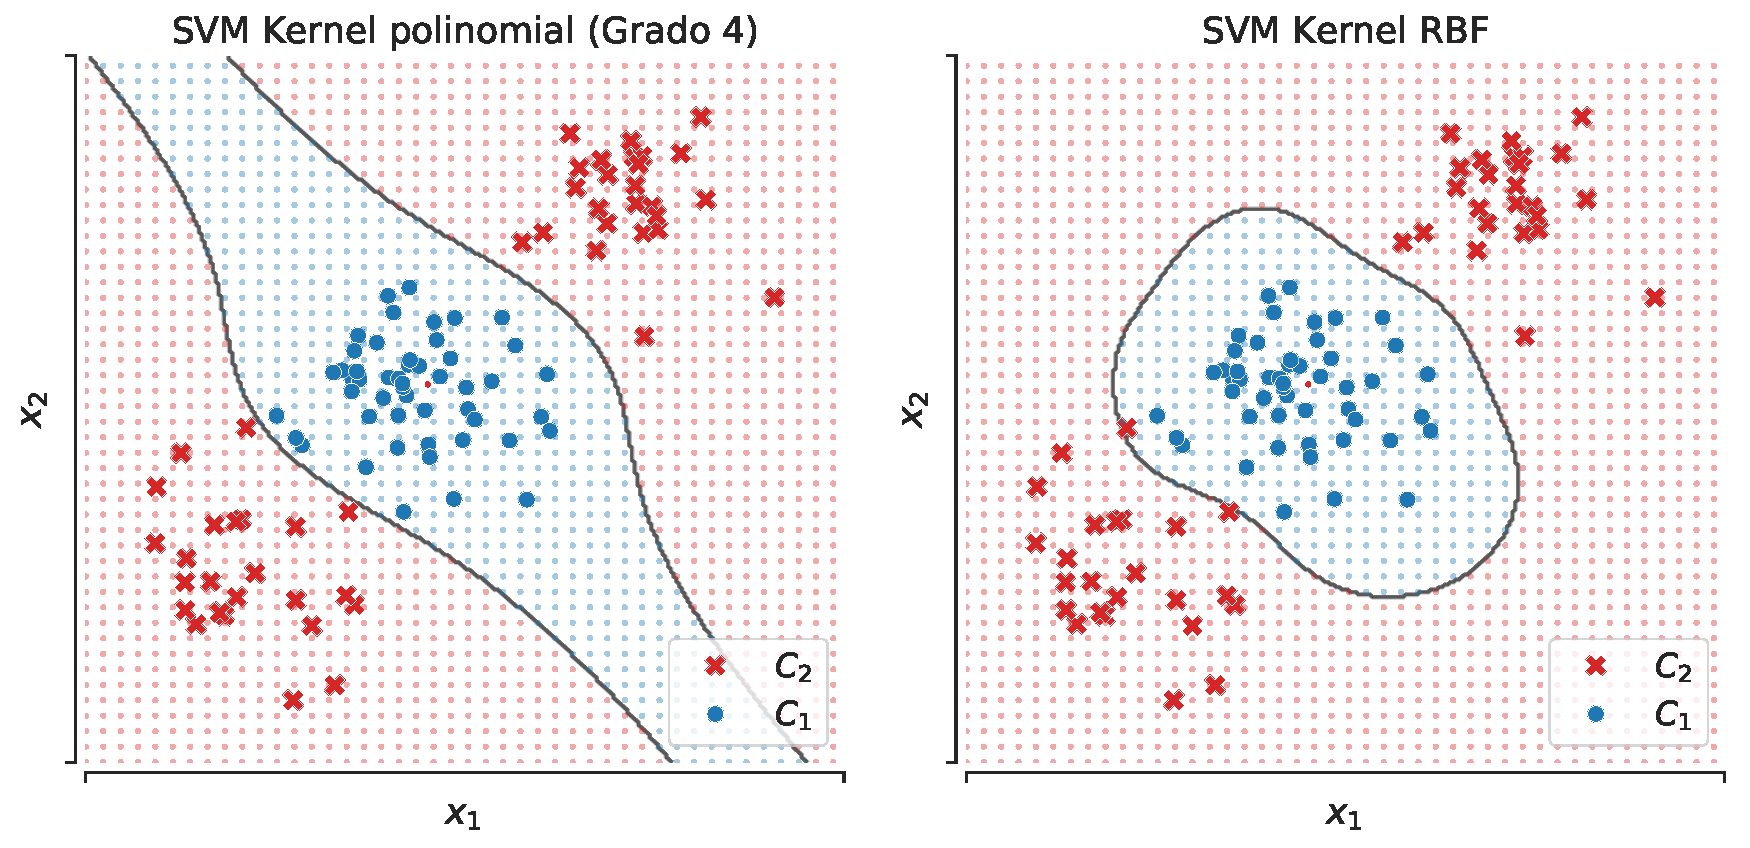
\includegraphics[width=0.8\textwidth]{img/cap5_svm_2kernels}
    \caption{Clasificación con distinto kernels.}
    \label{im:ca5_im6}
\end{figure}

A la izquierda se ocupo un kernel polinomial de grado $3$, dicho kernel permite un poco mas de curvatura en los límites del clasificador. A la derecha se ocupó un kernel RBF, el cual es capaz de encontrar fronteras de decisión más curvadas (Pero infinitamente diferenciables). 

Tener en cuenta que esta manera de resolver el problema tiene una tremenda ventaja computacional. Mover los datos a un espacio más grande mediante explícitamente definiendo $\phi(x)$, puede ser muy costoso, o incluso imposible en el caso que el espacio de llegada sea infinitamente dimensional. Usando funciones kernel dicha función queda implícita en el problema, dejandonos incluso trabajar en el caso infinito-dimensional (En el caso de RBF por ejemplo)


%-Comparar rendimiento de logistic regression c on SVM lineal
%-Usar diferentes Kernels
%-Ver el overfitting cuando ocupas un polinomio de muchos grados
%-Ver la importancia de escalar los datos


